% *** Pourquoi la réduction de dimension, et la décorellation des données.
% Cours Réda
% *** Pourquoi la LDA est insuffisante.
% Histoire des matrices de covariance.
% *** En quoi la HLDA résout le problème
% Ce qu'elle permet

\section{Introduction}
\label{sec:introduction}

In this state of the art, we will present a reduction-dimension method
which is a generalization of the LDA. There is several hypothesis to
be able to apply the LDA. We will present a case where we are
limited because all the hypothesis are not respected. And we will
introduce a method which is able to solve this kind of problem. This
method is the ``Heteroscedastic Linear Discriminant Analysis'' (HLDA).

FIXME: I need to know the exact plan to know what to say here...

\subsection{Limitations of the LDA}
\label{sec:limitations-lda}

One of the hypothesis made by the LDA is that the class distributions
are Gaussians with common covariance (Homoscedastic) and their means
lies in a subspace of the feature space. So, what is the behavior of
the method when the within-class distributions are heteroscedastic
(not homoscedastic)?

Let's take an example with only two classes where the means are
similar but they have very different distributions. We'll see in the
figure \ref{fig:lda-fail} this case.

\begin{figure}[h]
  \centering
  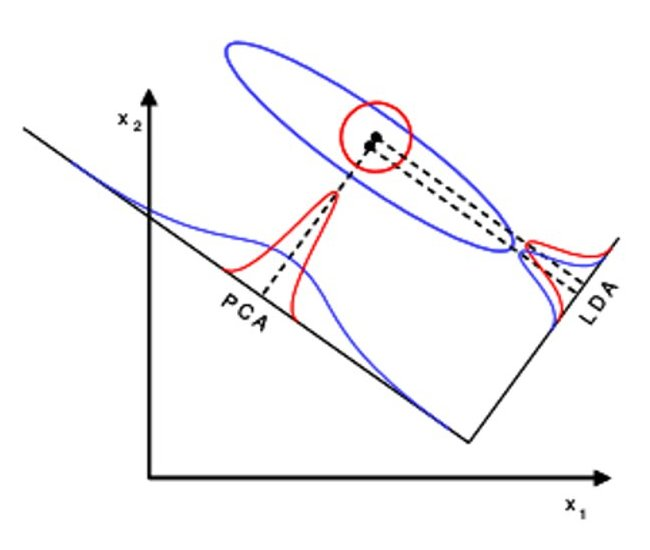
\includegraphics[scale=0.5]{img/limitation_lda}
%% FIXME: Try to change the img.
%%        Is it really a PCA in the other side of the LDA?
  \caption{Two classes with similar means and different distributions}
  \label{fig:lda-fail}
\end{figure}

Let's call the red class the A class, and the blue one the B. The mean
of A and the mean of B are very close. They are just a slight
translation in one direction, and the LDA will project the data on the
side marked as ``LDA''. And obviously, this is not the good choice.

In the literature, there is several proposition to solve this problem.
The HLDA is one of them. This method is presented in the thesis of
Kumar \cite{kumar.1997}. The method is described in the part
FIXME\_GARY. The solution proposed consists in modeling the data with a
heteroscedastic model.

